\documentclass[]{article}
\usepackage{lmodern}
\usepackage{amssymb,amsmath}
\usepackage{ifxetex,ifluatex}
\usepackage{fixltx2e} % provides \textsubscript
\ifnum 0\ifxetex 1\fi\ifluatex 1\fi=0 % if pdftex
  \usepackage[T1]{fontenc}
  \usepackage[utf8]{inputenc}
\else % if luatex or xelatex
  \ifxetex
    \usepackage{mathspec}
  \else
    \usepackage{fontspec}
  \fi
  \defaultfontfeatures{Ligatures=TeX,Scale=MatchLowercase}
\fi
% use upquote if available, for straight quotes in verbatim environments
\IfFileExists{upquote.sty}{\usepackage{upquote}}{}
% use microtype if available
\IfFileExists{microtype.sty}{%
\usepackage{microtype}
\UseMicrotypeSet[protrusion]{basicmath} % disable protrusion for tt fonts
}{}
\usepackage[margin=1in]{geometry}
\usepackage{hyperref}
\hypersetup{unicode=true,
            pdftitle={Reproducible Research: Peer Assessment 1},
            pdfauthor={Luis Fernando Agottani},
            pdfborder={0 0 0},
            breaklinks=true}
\urlstyle{same}  % don't use monospace font for urls
\usepackage{color}
\usepackage{fancyvrb}
\newcommand{\VerbBar}{|}
\newcommand{\VERB}{\Verb[commandchars=\\\{\}]}
\DefineVerbatimEnvironment{Highlighting}{Verbatim}{commandchars=\\\{\}}
% Add ',fontsize=\small' for more characters per line
\usepackage{framed}
\definecolor{shadecolor}{RGB}{248,248,248}
\newenvironment{Shaded}{\begin{snugshade}}{\end{snugshade}}
\newcommand{\AlertTok}[1]{\textcolor[rgb]{0.94,0.16,0.16}{#1}}
\newcommand{\AnnotationTok}[1]{\textcolor[rgb]{0.56,0.35,0.01}{\textbf{\textit{#1}}}}
\newcommand{\AttributeTok}[1]{\textcolor[rgb]{0.77,0.63,0.00}{#1}}
\newcommand{\BaseNTok}[1]{\textcolor[rgb]{0.00,0.00,0.81}{#1}}
\newcommand{\BuiltInTok}[1]{#1}
\newcommand{\CharTok}[1]{\textcolor[rgb]{0.31,0.60,0.02}{#1}}
\newcommand{\CommentTok}[1]{\textcolor[rgb]{0.56,0.35,0.01}{\textit{#1}}}
\newcommand{\CommentVarTok}[1]{\textcolor[rgb]{0.56,0.35,0.01}{\textbf{\textit{#1}}}}
\newcommand{\ConstantTok}[1]{\textcolor[rgb]{0.00,0.00,0.00}{#1}}
\newcommand{\ControlFlowTok}[1]{\textcolor[rgb]{0.13,0.29,0.53}{\textbf{#1}}}
\newcommand{\DataTypeTok}[1]{\textcolor[rgb]{0.13,0.29,0.53}{#1}}
\newcommand{\DecValTok}[1]{\textcolor[rgb]{0.00,0.00,0.81}{#1}}
\newcommand{\DocumentationTok}[1]{\textcolor[rgb]{0.56,0.35,0.01}{\textbf{\textit{#1}}}}
\newcommand{\ErrorTok}[1]{\textcolor[rgb]{0.64,0.00,0.00}{\textbf{#1}}}
\newcommand{\ExtensionTok}[1]{#1}
\newcommand{\FloatTok}[1]{\textcolor[rgb]{0.00,0.00,0.81}{#1}}
\newcommand{\FunctionTok}[1]{\textcolor[rgb]{0.00,0.00,0.00}{#1}}
\newcommand{\ImportTok}[1]{#1}
\newcommand{\InformationTok}[1]{\textcolor[rgb]{0.56,0.35,0.01}{\textbf{\textit{#1}}}}
\newcommand{\KeywordTok}[1]{\textcolor[rgb]{0.13,0.29,0.53}{\textbf{#1}}}
\newcommand{\NormalTok}[1]{#1}
\newcommand{\OperatorTok}[1]{\textcolor[rgb]{0.81,0.36,0.00}{\textbf{#1}}}
\newcommand{\OtherTok}[1]{\textcolor[rgb]{0.56,0.35,0.01}{#1}}
\newcommand{\PreprocessorTok}[1]{\textcolor[rgb]{0.56,0.35,0.01}{\textit{#1}}}
\newcommand{\RegionMarkerTok}[1]{#1}
\newcommand{\SpecialCharTok}[1]{\textcolor[rgb]{0.00,0.00,0.00}{#1}}
\newcommand{\SpecialStringTok}[1]{\textcolor[rgb]{0.31,0.60,0.02}{#1}}
\newcommand{\StringTok}[1]{\textcolor[rgb]{0.31,0.60,0.02}{#1}}
\newcommand{\VariableTok}[1]{\textcolor[rgb]{0.00,0.00,0.00}{#1}}
\newcommand{\VerbatimStringTok}[1]{\textcolor[rgb]{0.31,0.60,0.02}{#1}}
\newcommand{\WarningTok}[1]{\textcolor[rgb]{0.56,0.35,0.01}{\textbf{\textit{#1}}}}
\usepackage{graphicx,grffile}
\makeatletter
\def\maxwidth{\ifdim\Gin@nat@width>\linewidth\linewidth\else\Gin@nat@width\fi}
\def\maxheight{\ifdim\Gin@nat@height>\textheight\textheight\else\Gin@nat@height\fi}
\makeatother
% Scale images if necessary, so that they will not overflow the page
% margins by default, and it is still possible to overwrite the defaults
% using explicit options in \includegraphics[width, height, ...]{}
\setkeys{Gin}{width=\maxwidth,height=\maxheight,keepaspectratio}
\IfFileExists{parskip.sty}{%
\usepackage{parskip}
}{% else
\setlength{\parindent}{0pt}
\setlength{\parskip}{6pt plus 2pt minus 1pt}
}
\setlength{\emergencystretch}{3em}  % prevent overfull lines
\providecommand{\tightlist}{%
  \setlength{\itemsep}{0pt}\setlength{\parskip}{0pt}}
\setcounter{secnumdepth}{0}
% Redefines (sub)paragraphs to behave more like sections
\ifx\paragraph\undefined\else
\let\oldparagraph\paragraph
\renewcommand{\paragraph}[1]{\oldparagraph{#1}\mbox{}}
\fi
\ifx\subparagraph\undefined\else
\let\oldsubparagraph\subparagraph
\renewcommand{\subparagraph}[1]{\oldsubparagraph{#1}\mbox{}}
\fi

%%% Use protect on footnotes to avoid problems with footnotes in titles
\let\rmarkdownfootnote\footnote%
\def\footnote{\protect\rmarkdownfootnote}

%%% Change title format to be more compact
\usepackage{titling}

% Create subtitle command for use in maketitle
\providecommand{\subtitle}[1]{
  \posttitle{
    \begin{center}\large#1\end{center}
    }
}

\setlength{\droptitle}{-2em}

  \title{Reproducible Research: Peer Assessment 1}
    \pretitle{\vspace{\droptitle}\centering\huge}
  \posttitle{\par}
    \author{Luis Fernando Agottani}
    \preauthor{\centering\large\emph}
  \postauthor{\par}
      \predate{\centering\large\emph}
  \postdate{\par}
    \date{09/08/2019}


\begin{document}
\maketitle

\hypertarget{loading-and-preprocessing-the-data}{%
\subsection{Loading and preprocessing the
data}\label{loading-and-preprocessing-the-data}}

Verify if the filename has been downloaded/unzip yet. If not,
download/unzip the file with the fileURL link.

\begin{Shaded}
\begin{Highlighting}[]
\NormalTok{filename <-}\StringTok{ "repdata_data_activity.zip"}

\ControlFlowTok{if}\NormalTok{ (}\OperatorTok{!}\KeywordTok{file.exists}\NormalTok{(filename))\{}
\NormalTok{  fileURL <-}\StringTok{ "https://d396qusza40orc.cloudfront.net/repdata%2Fdata%2Factivity.zip"}
  \KeywordTok{download.file}\NormalTok{(fileURL, filename)}
\NormalTok{\}}
\ControlFlowTok{if}\NormalTok{ (}\OperatorTok{!}\KeywordTok{file.exists}\NormalTok{(}\StringTok{"activity.csv"}\NormalTok{)) \{ }
  \KeywordTok{unzip}\NormalTok{(filename)}
\NormalTok{\}}
\end{Highlighting}
\end{Shaded}

Reading data.csv.

\begin{Shaded}
\begin{Highlighting}[]
\NormalTok{Act<-}\StringTok{ }\KeywordTok{read.csv}\NormalTok{(}\StringTok{"activity.csv"}\NormalTok{, }
               \DataTypeTok{head =} \OtherTok{TRUE}\NormalTok{, }\DataTypeTok{sep=} \StringTok{","}\NormalTok{)}
\end{Highlighting}
\end{Shaded}

Changing the Factor type of the column date to Date with as.Date.

\begin{Shaded}
\begin{Highlighting}[]
\NormalTok{Act}\OperatorTok{$}\NormalTok{date<-}\StringTok{ }\KeywordTok{as.Date}\NormalTok{(Act}\OperatorTok{$}\NormalTok{date)}
\end{Highlighting}
\end{Shaded}

\hypertarget{what-is-mean-total-number-of-steps-taken-per-day}{%
\subsection{What is mean total number of steps taken per
day?}\label{what-is-mean-total-number-of-steps-taken-per-day}}

Library Dplyr to work with ``\%\textgreater{}\%''

\begin{Shaded}
\begin{Highlighting}[]
\KeywordTok{library}\NormalTok{(dplyr)}
\end{Highlighting}
\end{Shaded}

The total number of steps is the sum of all steps measured by day. The
mean is the sum divided by the number of intervals..

\begin{Shaded}
\begin{Highlighting}[]
\NormalTok{Act_Day<-}\StringTok{ }\NormalTok{Act }\OperatorTok\StringTok{ }
\StringTok{  }\KeywordTok{group_by}\NormalTok{(date) }\OperatorTok\StringTok{ }
\StringTok{  }\KeywordTok{summarise}\NormalTok{(}\DataTypeTok{steps =} \KeywordTok{sum}\NormalTok{(steps))}
\end{Highlighting}
\end{Shaded}

\hypertarget{including-plots}{%
\subsection{Including Plots}\label{including-plots}}

Ploting a histogram with the sum, mean and median of steps by day.

\begin{Shaded}
\begin{Highlighting}[]
\KeywordTok{hist}\NormalTok{(Act_Day}\OperatorTok{$}\NormalTok{steps, }
     \DataTypeTok{breaks=} \KeywordTok{seq}\NormalTok{(}\DataTypeTok{from=}\DecValTok{0}\NormalTok{, }\DataTypeTok{to=}\DecValTok{25000}\NormalTok{, }\DataTypeTok{by=}\DecValTok{2500}\NormalTok{), }
     \DataTypeTok{col=}\StringTok{"darkblue"}\NormalTok{, }
     \DataTypeTok{border=}\StringTok{"black"}\NormalTok{, }
     \DataTypeTok{xlab=}\StringTok{"Number of Steps"}\NormalTok{, }
     \DataTypeTok{main=}\StringTok{"Mean and Median of the total number of steps by day"}\NormalTok{, }
     \DataTypeTok{ylim=}\KeywordTok{c}\NormalTok{(}\DecValTok{0}\NormalTok{, }\DecValTok{20}\NormalTok{),}
     \DataTypeTok{xlim=}\KeywordTok{c}\NormalTok{(}\DecValTok{0}\NormalTok{,}\DecValTok{25000}\NormalTok{))}

\KeywordTok{abline}\NormalTok{(}\DataTypeTok{v=}\KeywordTok{median}\NormalTok{(Act_Day}\OperatorTok{$}\NormalTok{steps,}
                \DataTypeTok{na.rm=}\OtherTok{TRUE}\NormalTok{), }
       \DataTypeTok{col=}\StringTok{"green"}\NormalTok{,}
       \DataTypeTok{lwd=}\DecValTok{4}\NormalTok{)}

\KeywordTok{abline}\NormalTok{(}\DataTypeTok{v=}\KeywordTok{mean}\NormalTok{(Act_Day}\OperatorTok{$}\NormalTok{steps, }
              \DataTypeTok{na.rm=}\OtherTok{TRUE}\NormalTok{), }
       \DataTypeTok{col=}\StringTok{"red"}\NormalTok{,}\DataTypeTok{lwd=}\DecValTok{2}\NormalTok{)}

\KeywordTok{legend}\NormalTok{(}\DataTypeTok{x=}\StringTok{"topright"}\NormalTok{, }\CommentTok{#subtitle postion}
      \KeywordTok{c}\NormalTok{(}\StringTok{"Median"}\NormalTok{,}\StringTok{"Mean"}\NormalTok{), }\CommentTok{#name of the subtitle}
      \DataTypeTok{col=}\KeywordTok{c}\NormalTok{(}\StringTok{"green"}\NormalTok{,}\StringTok{"red"}\NormalTok{), }\CommentTok{#colors}
      \DataTypeTok{lty=}\KeywordTok{c}\NormalTok{(}\DecValTok{1}\NormalTok{,}\DecValTok{1}\NormalTok{), }\CommentTok{#line style}
      \DataTypeTok{lwd=}\KeywordTok{c}\NormalTok{(}\DecValTok{4}\NormalTok{,}\DecValTok{2}\NormalTok{)) }\CommentTok{#line widht}
\end{Highlighting}
\end{Shaded}

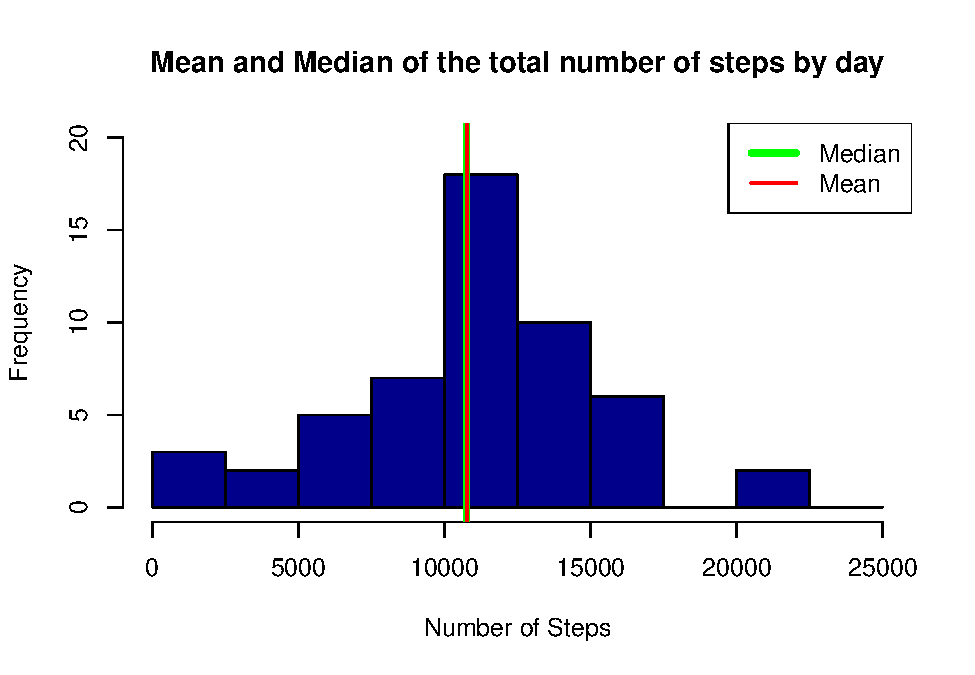
\includegraphics{PA1_template_files/figure-latex/ploting 1 -1.pdf}

\hypertarget{what-is-the-average-daily-activity-pattern}{%
\subsection{What is the average daily activity
pattern?}\label{what-is-the-average-daily-activity-pattern}}

The daily activity pattern is the mean of the number of steps of all
days by interval.

\begin{Shaded}
\begin{Highlighting}[]
\NormalTok{Act_Interval<-}\StringTok{ }\NormalTok{Act }\OperatorTok\StringTok{ }
\StringTok{  }\KeywordTok{group_by}\NormalTok{(interval) }\OperatorTok\StringTok{ }
\StringTok{  }\KeywordTok{summarise}\NormalTok{(}\DataTypeTok{steps =} \KeywordTok{mean}\NormalTok{(steps, }
                         \DataTypeTok{na.rm=}\OtherTok{TRUE}\NormalTok{))}
\end{Highlighting}
\end{Shaded}

Ploting the Mean of steps of all days by Interval with the line plot.

\begin{Shaded}
\begin{Highlighting}[]
\KeywordTok{plot}\NormalTok{(Act_Interval}\OperatorTok{$}\NormalTok{interval, }
\NormalTok{     Act_Interval}\OperatorTok{$}\NormalTok{steps, }
     \DataTypeTok{type=}\StringTok{"l"}\NormalTok{, }
     \DataTypeTok{col=}\StringTok{"darkblue"}\NormalTok{, }
     \DataTypeTok{xlab=}\StringTok{"Interval(Minute)"}\NormalTok{, }
     \DataTypeTok{ylab=}\StringTok{"Mean of steps"}\NormalTok{, }
     \DataTypeTok{main=}\StringTok{"The daily activity pattern"}\NormalTok{)}

\KeywordTok{abline}\NormalTok{(}\DataTypeTok{h=}\KeywordTok{max}\NormalTok{(Act_Interval}\OperatorTok{$}\NormalTok{steps),}
       \DataTypeTok{col=}\StringTok{"green"}\NormalTok{,}
       \DataTypeTok{lwd=}\DecValTok{2}\NormalTok{)}

\KeywordTok{legend}\NormalTok{(}\DataTypeTok{x=}\StringTok{"topright"}\NormalTok{,}
      \StringTok{"Valor máximo"}\NormalTok{,}
      \DataTypeTok{col=}\StringTok{"green"}\NormalTok{,}
      \DataTypeTok{lty=}\DecValTok{1}\NormalTok{,}
      \DataTypeTok{lwd=}\DecValTok{2}\NormalTok{)}
\end{Highlighting}
\end{Shaded}

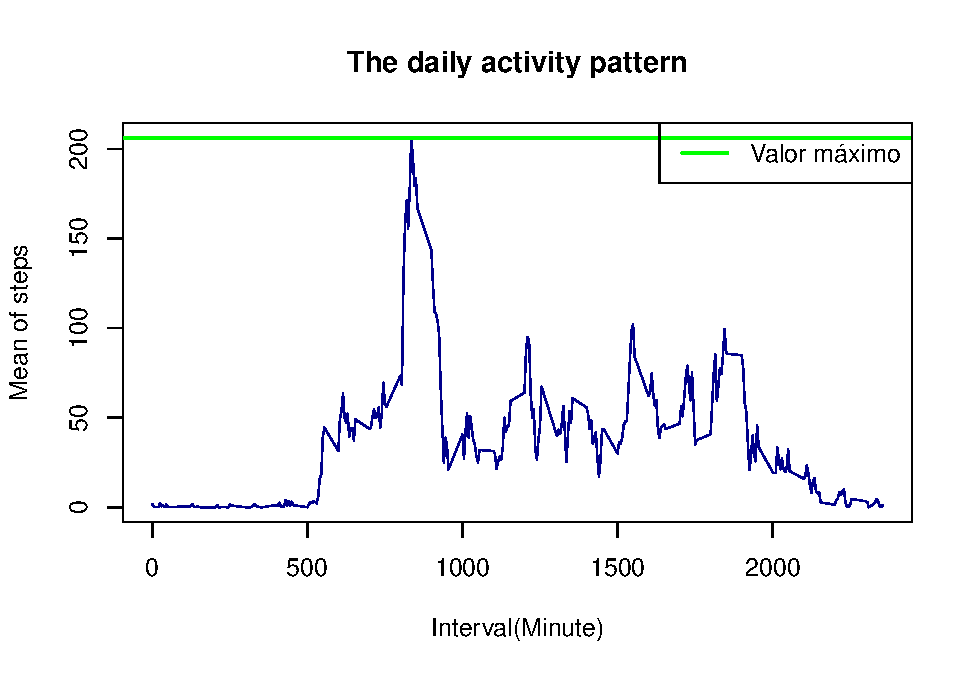
\includegraphics{PA1_template_files/figure-latex/ploting 2-1.pdf}

\hypertarget{imputing-missing-values}{%
\subsection{Imputing missing values}\label{imputing-missing-values}}

To represent the missing data and verify the number of the missing data
in each column, a nice way to do it is with the package ``mice'' and
``VIM''.

\begin{Shaded}
\begin{Highlighting}[]
\KeywordTok{library}\NormalTok{(mice)}
\KeywordTok{library}\NormalTok{(VIM)}

\NormalTok{mice_plot <-}\StringTok{ }\KeywordTok{aggr}\NormalTok{(Act_Day, }
                  \DataTypeTok{col=}\KeywordTok{c}\NormalTok{(}\StringTok{'navyblue'}\NormalTok{,}\StringTok{'yellow'}\NormalTok{),}
                  \DataTypeTok{numbers=}\OtherTok{TRUE}\NormalTok{, }
                  \DataTypeTok{sortVars=}\OtherTok{TRUE}\NormalTok{,}
                  \DataTypeTok{labels=}\KeywordTok{names}\NormalTok{(Act_Day), }
                  \DataTypeTok{cex.axis=}\NormalTok{.}\DecValTok{7}\NormalTok{,}
                  \DataTypeTok{gap=}\DecValTok{3}\NormalTok{, }
                  \DataTypeTok{ylab=}\KeywordTok{c}\NormalTok{(}\StringTok{"Missing data"}\NormalTok{,}\StringTok{"Pattern"}\NormalTok{))}
\end{Highlighting}
\end{Shaded}

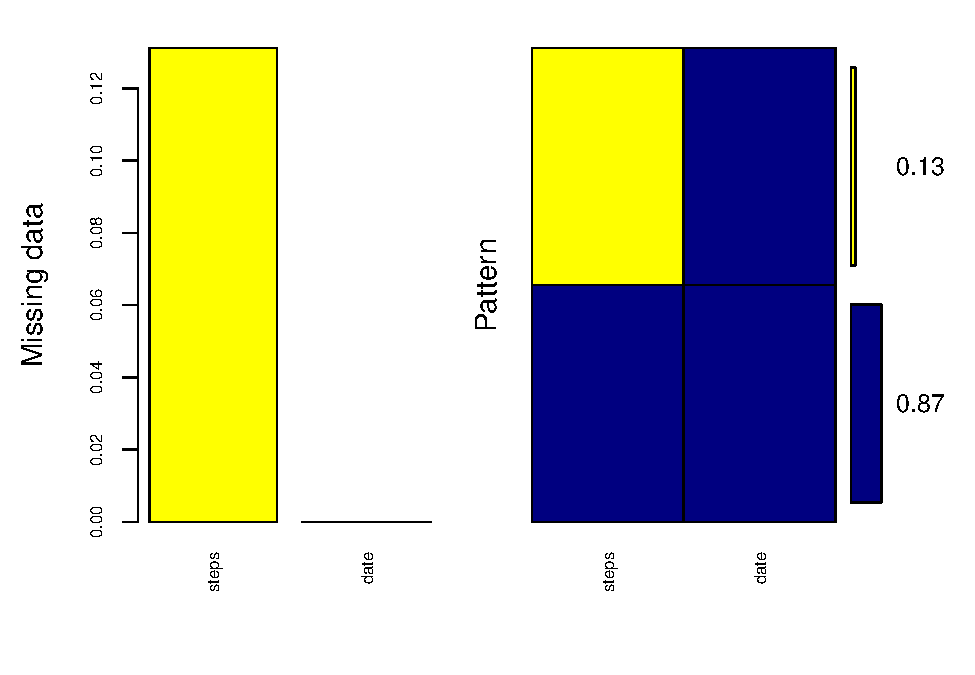
\includegraphics{PA1_template_files/figure-latex/Counting missing data-1.pdf}

\begin{verbatim}
## 
##  Variables sorted by number of missings: 
##  Variable     Count
##     steps 0.1311475
##      date 0.0000000
\end{verbatim}

The result show us that is a big amount, x\textgreater{}5\%, of NA's in
the data, we have to take care to impute the a value that help us with
accuracy.

With library ``mice'' and the pmm method, we will impute values to
missing data.

\begin{Shaded}
\begin{Highlighting}[]
\NormalTok{imputed_Data <-}\StringTok{ }\KeywordTok{mice}\NormalTok{(Act, }
                     \DataTypeTok{m=}\DecValTok{5}\NormalTok{, }
                     \DataTypeTok{maxit =} \DecValTok{50}\NormalTok{, }
                     \DataTypeTok{method =} \StringTok{'pmm'}\NormalTok{, }
                     \DataTypeTok{seed =} \DecValTok{500}\NormalTok{)}
\end{Highlighting}
\end{Shaded}

\begin{verbatim}
## 
##  iter imp variable
##   1   1  steps
##   1   2  steps
##   1   3  steps
##   1   4  steps
##   1   5  steps
##   2   1  steps
##   2   2  steps
##   2   3  steps
##   2   4  steps
##   2   5  steps
##   3   1  steps
##   3   2  steps
##   3   3  steps
##   3   4  steps
##   3   5  steps
##   4   1  steps
##   4   2  steps
##   4   3  steps
##   4   4  steps
##   4   5  steps
##   5   1  steps
##   5   2  steps
##   5   3  steps
##   5   4  steps
##   5   5  steps
##   6   1  steps
##   6   2  steps
##   6   3  steps
##   6   4  steps
##   6   5  steps
##   7   1  steps
##   7   2  steps
##   7   3  steps
##   7   4  steps
##   7   5  steps
##   8   1  steps
##   8   2  steps
##   8   3  steps
##   8   4  steps
##   8   5  steps
##   9   1  steps
##   9   2  steps
##   9   3  steps
##   9   4  steps
##   9   5  steps
##   10   1  steps
##   10   2  steps
##   10   3  steps
##   10   4  steps
##   10   5  steps
##   11   1  steps
##   11   2  steps
##   11   3  steps
##   11   4  steps
##   11   5  steps
##   12   1  steps
##   12   2  steps
##   12   3  steps
##   12   4  steps
##   12   5  steps
##   13   1  steps
##   13   2  steps
##   13   3  steps
##   13   4  steps
##   13   5  steps
##   14   1  steps
##   14   2  steps
##   14   3  steps
##   14   4  steps
##   14   5  steps
##   15   1  steps
##   15   2  steps
##   15   3  steps
##   15   4  steps
##   15   5  steps
##   16   1  steps
##   16   2  steps
##   16   3  steps
##   16   4  steps
##   16   5  steps
##   17   1  steps
##   17   2  steps
##   17   3  steps
##   17   4  steps
##   17   5  steps
##   18   1  steps
##   18   2  steps
##   18   3  steps
##   18   4  steps
##   18   5  steps
##   19   1  steps
##   19   2  steps
##   19   3  steps
##   19   4  steps
##   19   5  steps
##   20   1  steps
##   20   2  steps
##   20   3  steps
##   20   4  steps
##   20   5  steps
##   21   1  steps
##   21   2  steps
##   21   3  steps
##   21   4  steps
##   21   5  steps
##   22   1  steps
##   22   2  steps
##   22   3  steps
##   22   4  steps
##   22   5  steps
##   23   1  steps
##   23   2  steps
##   23   3  steps
##   23   4  steps
##   23   5  steps
##   24   1  steps
##   24   2  steps
##   24   3  steps
##   24   4  steps
##   24   5  steps
##   25   1  steps
##   25   2  steps
##   25   3  steps
##   25   4  steps
##   25   5  steps
##   26   1  steps
##   26   2  steps
##   26   3  steps
##   26   4  steps
##   26   5  steps
##   27   1  steps
##   27   2  steps
##   27   3  steps
##   27   4  steps
##   27   5  steps
##   28   1  steps
##   28   2  steps
##   28   3  steps
##   28   4  steps
##   28   5  steps
##   29   1  steps
##   29   2  steps
##   29   3  steps
##   29   4  steps
##   29   5  steps
##   30   1  steps
##   30   2  steps
##   30   3  steps
##   30   4  steps
##   30   5  steps
##   31   1  steps
##   31   2  steps
##   31   3  steps
##   31   4  steps
##   31   5  steps
##   32   1  steps
##   32   2  steps
##   32   3  steps
##   32   4  steps
##   32   5  steps
##   33   1  steps
##   33   2  steps
##   33   3  steps
##   33   4  steps
##   33   5  steps
##   34   1  steps
##   34   2  steps
##   34   3  steps
##   34   4  steps
##   34   5  steps
##   35   1  steps
##   35   2  steps
##   35   3  steps
##   35   4  steps
##   35   5  steps
##   36   1  steps
##   36   2  steps
##   36   3  steps
##   36   4  steps
##   36   5  steps
##   37   1  steps
##   37   2  steps
##   37   3  steps
##   37   4  steps
##   37   5  steps
##   38   1  steps
##   38   2  steps
##   38   3  steps
##   38   4  steps
##   38   5  steps
##   39   1  steps
##   39   2  steps
##   39   3  steps
##   39   4  steps
##   39   5  steps
##   40   1  steps
##   40   2  steps
##   40   3  steps
##   40   4  steps
##   40   5  steps
##   41   1  steps
##   41   2  steps
##   41   3  steps
##   41   4  steps
##   41   5  steps
##   42   1  steps
##   42   2  steps
##   42   3  steps
##   42   4  steps
##   42   5  steps
##   43   1  steps
##   43   2  steps
##   43   3  steps
##   43   4  steps
##   43   5  steps
##   44   1  steps
##   44   2  steps
##   44   3  steps
##   44   4  steps
##   44   5  steps
##   45   1  steps
##   45   2  steps
##   45   3  steps
##   45   4  steps
##   45   5  steps
##   46   1  steps
##   46   2  steps
##   46   3  steps
##   46   4  steps
##   46   5  steps
##   47   1  steps
##   47   2  steps
##   47   3  steps
##   47   4  steps
##   47   5  steps
##   48   1  steps
##   48   2  steps
##   48   3  steps
##   48   4  steps
##   48   5  steps
##   49   1  steps
##   49   2  steps
##   49   3  steps
##   49   4  steps
##   49   5  steps
##   50   1  steps
##   50   2  steps
##   50   3  steps
##   50   4  steps
##   50   5  steps
\end{verbatim}

\begin{Shaded}
\begin{Highlighting}[]
\NormalTok{completeData <-}\StringTok{ }\KeywordTok{complete}\NormalTok{(imputed_Data,}\DecValTok{2}\NormalTok{)}

\NormalTok{completeDataSum<-}\StringTok{ }\NormalTok{completeData }\OperatorTok\StringTok{ }
\StringTok{  }\KeywordTok{group_by}\NormalTok{(date) }\OperatorTok\StringTok{ }
\StringTok{  }\KeywordTok{summarise}\NormalTok{(}\DataTypeTok{steps =} \KeywordTok{sum}\NormalTok{(steps))}
\end{Highlighting}
\end{Shaded}

Ploting the complete data.

\begin{Shaded}
\begin{Highlighting}[]
\KeywordTok{hist}\NormalTok{(completeDataSum}\OperatorTok{$}\NormalTok{steps, }
     \DataTypeTok{breaks=} \KeywordTok{seq}\NormalTok{(}\DataTypeTok{from=}\DecValTok{0}\NormalTok{, }\DataTypeTok{to=}\DecValTok{25000}\NormalTok{, }\DataTypeTok{by=}\DecValTok{2500}\NormalTok{), }
     \DataTypeTok{col=}\StringTok{"darkgreen"}\NormalTok{, }
     \DataTypeTok{border=}\StringTok{"black"}\NormalTok{, }
     \DataTypeTok{xlab=}\StringTok{"Number of Steps"}\NormalTok{, }
     \DataTypeTok{main=}\StringTok{"Mean and Median of the total number of steps by day"}\NormalTok{, }
     \DataTypeTok{ylim=}\KeywordTok{c}\NormalTok{(}\DecValTok{0}\NormalTok{, }\DecValTok{20}\NormalTok{),}
     \DataTypeTok{xlim=}\KeywordTok{c}\NormalTok{(}\DecValTok{0}\NormalTok{,}\DecValTok{25000}\NormalTok{))}
      

\KeywordTok{abline}\NormalTok{(}\DataTypeTok{v=}\KeywordTok{median}\NormalTok{(completeDataSum}\OperatorTok{$}\NormalTok{steps,}\DataTypeTok{na.rm=}\OtherTok{TRUE}\NormalTok{), }
       \DataTypeTok{col=}\StringTok{"blue"}\NormalTok{,}
       \DataTypeTok{lwd=}\DecValTok{4}\NormalTok{)}

\KeywordTok{abline}\NormalTok{(}\DataTypeTok{v=}\KeywordTok{mean}\NormalTok{(completeDataSum}\OperatorTok{$}\NormalTok{steps, }
              \DataTypeTok{na.rm=}\OtherTok{TRUE}\NormalTok{), }
       \DataTypeTok{col=}\StringTok{"red"}\NormalTok{,}
       \DataTypeTok{lwd=}\DecValTok{2}\NormalTok{)}

\KeywordTok{legend}\NormalTok{(}\DataTypeTok{x=}\StringTok{"topright"}\NormalTok{,}
      \KeywordTok{c}\NormalTok{(}\StringTok{"Median"}\NormalTok{,}\StringTok{"Mean"}\NormalTok{),}
      \DataTypeTok{col=}\KeywordTok{c}\NormalTok{(}\StringTok{"blue"}\NormalTok{,}\StringTok{"red"}\NormalTok{),}
      \DataTypeTok{lty=}\KeywordTok{c}\NormalTok{(}\DecValTok{1}\NormalTok{,}\DecValTok{1}\NormalTok{), }
      \DataTypeTok{lwd=}\KeywordTok{c}\NormalTok{(}\DecValTok{4}\NormalTok{,}\DecValTok{2}\NormalTok{)) }
\end{Highlighting}
\end{Shaded}

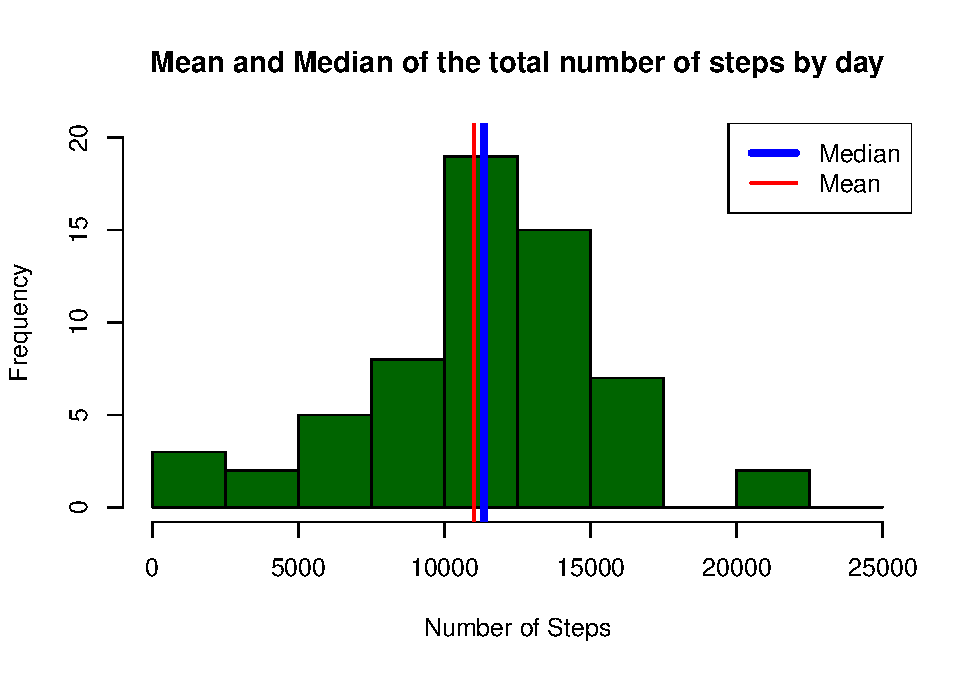
\includegraphics{PA1_template_files/figure-latex/ploting complete data-1.pdf}

As we can see, imputing values with de pmm method showed us a similar
result comparing with the first part of the assignment. So, we can
assume that imputing missing values did not impacted signifcally.

\hypertarget{are-there-differences-in-activity-patterns-between-weekdays-and-weekends}{%
\subsection{Are there differences in activity patterns between weekdays
and
weekends?}\label{are-there-differences-in-activity-patterns-between-weekdays-and-weekends}}

\begin{Shaded}
\begin{Highlighting}[]
\NormalTok{Act_days<-}\StringTok{ }\KeywordTok{mutate}\NormalTok{(completeData, }
                  \DataTypeTok{days=}\KeywordTok{weekdays}\NormalTok{(completeData}\OperatorTok{$}\NormalTok{date))}

\NormalTok{Act_week<-}\StringTok{ }\KeywordTok{mutate}\NormalTok{(Act_days,}
                  \DataTypeTok{weekpart=}\NormalTok{(}\KeywordTok{ifelse}\NormalTok{(Act_days}\OperatorTok{$}\NormalTok{days}\OperatorTok{==}\StringTok{"sábado"}\OperatorTok{|}\NormalTok{Act_days}\OperatorTok{$}\NormalTok{days}\OperatorTok{==}\StringTok{"domingo"}\NormalTok{,}\StringTok{"weekend"}\NormalTok{,}\StringTok{"weekday"}\NormalTok{)))}

\NormalTok{Act_weekdays<-}\StringTok{ }\NormalTok{Act_week }\OperatorTok\StringTok{ }
\StringTok{  }\KeywordTok{group_by}\NormalTok{(interval,weekpart) }\OperatorTok\StringTok{ }
\StringTok{  }\KeywordTok{summarise}\NormalTok{(}\DataTypeTok{steps =} \KeywordTok{mean}\NormalTok{(steps))}
\end{Highlighting}
\end{Shaded}

Ploting the comparassion between the parts of the week, ``weekdays'' and
``weekend'', to see if have some pattern there.

\begin{Shaded}
\begin{Highlighting}[]
\KeywordTok{library}\NormalTok{(ggplot2)}

\KeywordTok{ggplot}\NormalTok{(}\KeywordTok{aes}\NormalTok{(}\DataTypeTok{x=}\NormalTok{interval,}\DataTypeTok{y=}\NormalTok{steps),}
       \DataTypeTok{data=}\NormalTok{Act_weekdays)}\OperatorTok{+}
\StringTok{       }\KeywordTok{geom_line}\NormalTok{(}\DataTypeTok{col=}\StringTok{"blue"}\NormalTok{)}\OperatorTok{+}
\StringTok{       }\KeywordTok{facet_wrap}\NormalTok{(}\OperatorTok{~}\NormalTok{Act_weekdays}\OperatorTok{$}\NormalTok{weekpart)}
\end{Highlighting}
\end{Shaded}

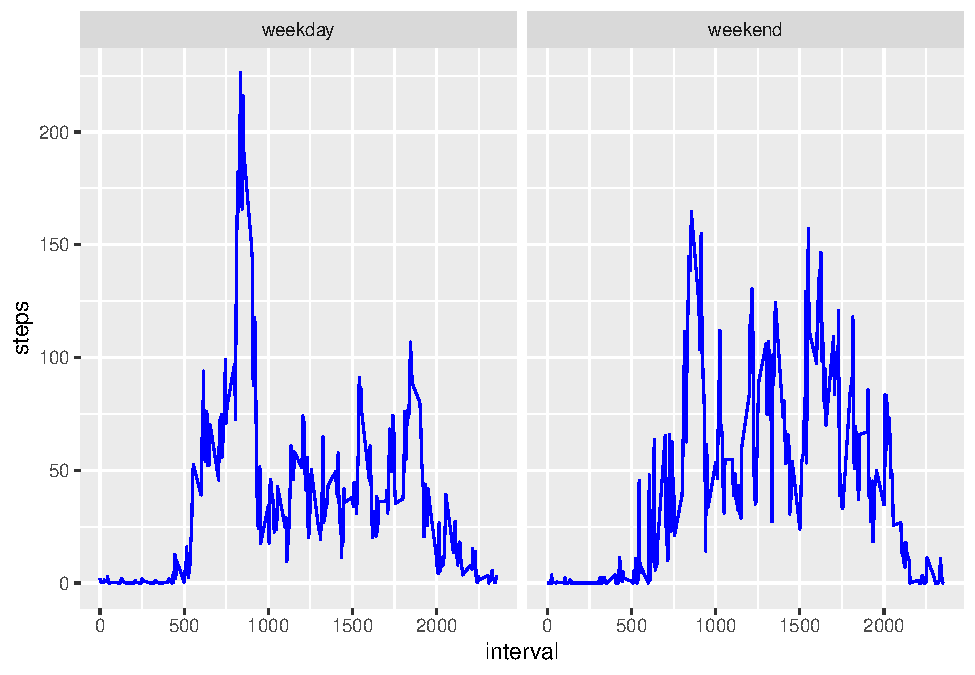
\includegraphics{PA1_template_files/figure-latex/ploting data to 2 levels-1.pdf}


\end{document}
